\documentclass[a4paper,12pt]{article}
\usepackage{tikz}
\usetikzlibrary{shapes.geometric, arrows}

\tikzstyle{startstop} = [rectangle, rounded corners, minimum width=3cm, minimum height=1cm,text centered, draw=black, fill=red!30]
\tikzstyle{process} = [rectangle, minimum width=3cm, minimum height=1cm, text centered, draw=black, fill=blue!20]
\tikzstyle{decision} = [diamond, minimum width=3cm, minimum height=1cm, text centered, draw=black, fill=green!30]
\tikzstyle{arrow} = [thick,->,>=stealth]

\usepackage{graphicx}
\usepackage{hyperref}
\usepackage{geometry}
\geometry{margin=1in}

\title{Spreadsheet Engine - C Lab}
\author{
    Prakhar Gupta \\ \small 2023CS10493 \and
    Keshav Bansal \\ \small 2023MT110273 \and
    Dhruv Pawar \\ \small 2023CS5230184
}

\date{\today}

\begin{document}

\maketitle

\section{Introduction}
This report provides an overview of the Spreadsheet Engine we have designed for the COP290 C lab. The program supports user interactions with a simple command-line interface and performs major Excel functionalities to a great extent.

\section{Structure}
The project follows a modular structure with key files integrating to build the whole project. Each file has its own function following a workflow, ensuring proper data handling and maximum efficiency. 

\subsection{Key Files}
\begin{itemize}
    \item \textbf{main} - Entry point of the application.
    \item \textbf{parser} - Translates user inputs with valid checks.
    \item \textbf{frontend} - Maintains the interface.
    \item \textbf{backend} - Handles computation and data storage.
    \item \textbf{structs, cell, and vec} - Various utility functions and data structures.
    \item \textbf{test directory} - Various tests handling all edge cases and functionalities, ensuring correctness.
    \item \textbf{README} - Short summary and guide for using the project.
    \item \textbf{Makefile} - Automates compilation and execution in the terminal.
\end{itemize}

\begin{center}
    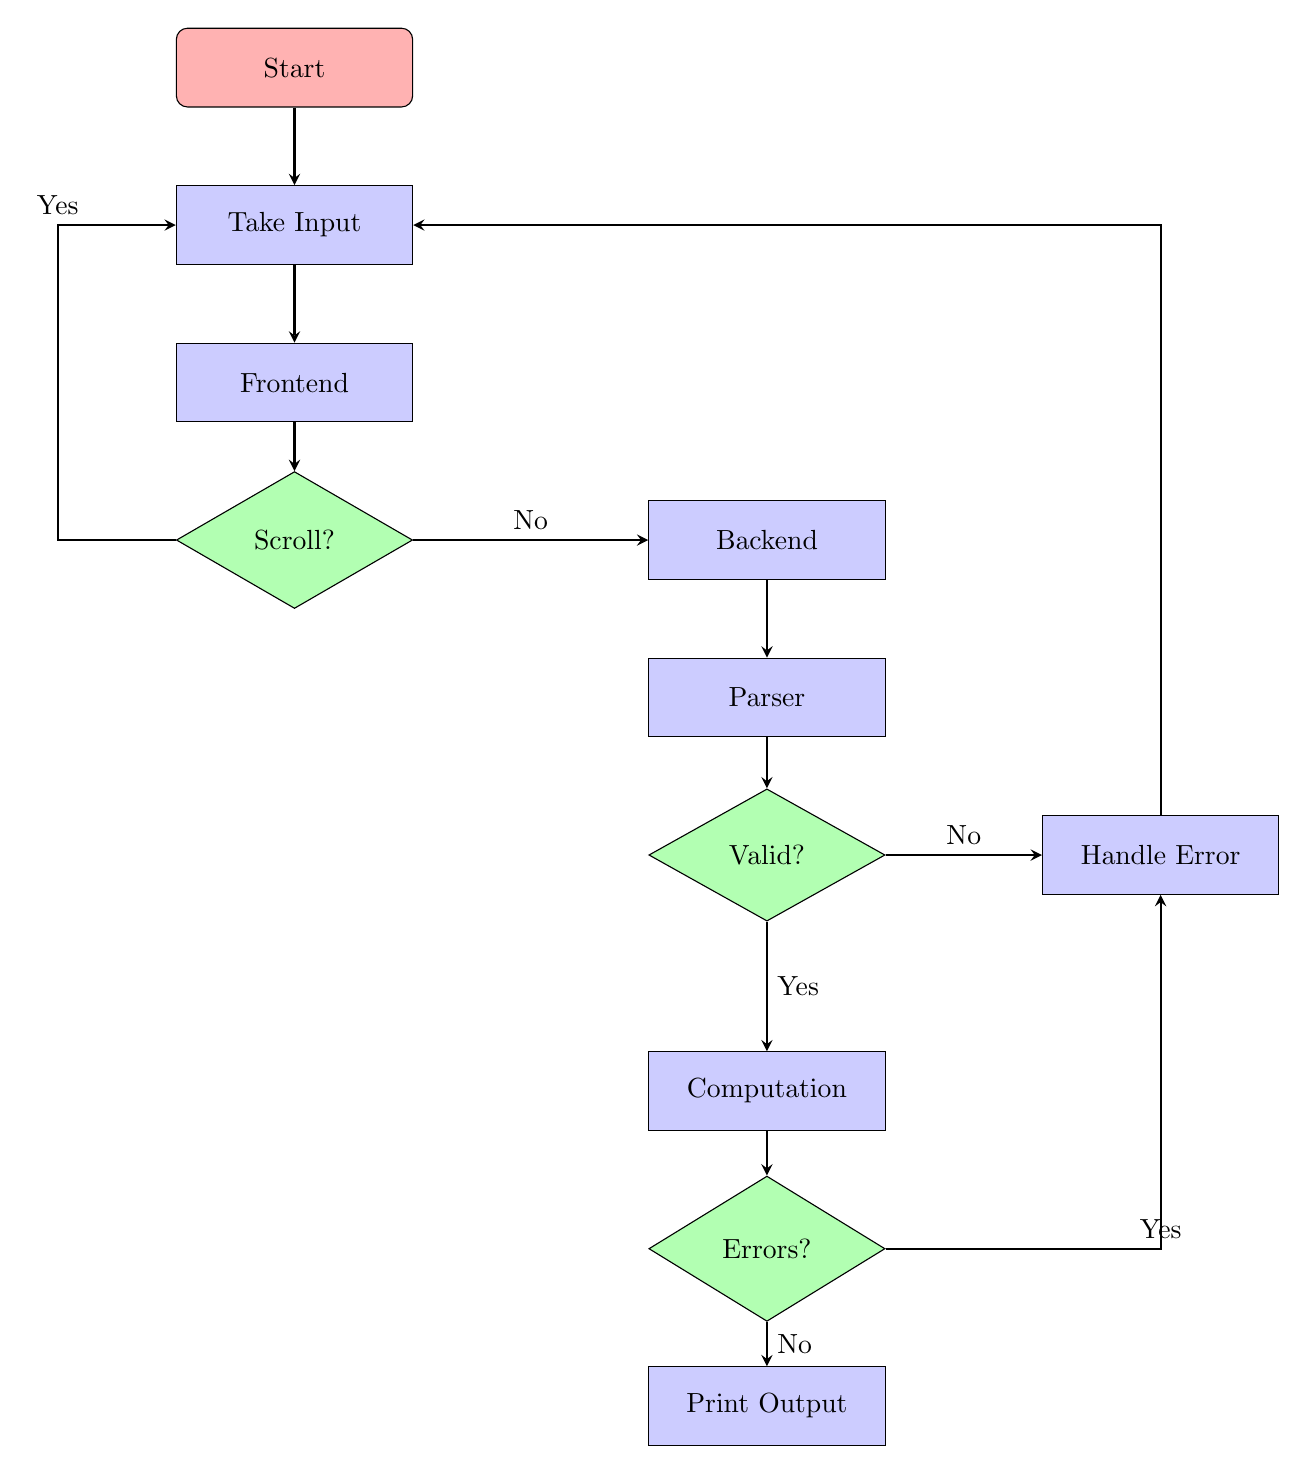
\begin{tikzpicture}[node distance=2cm]
        \node (start) [startstop] {Start};
        \node (input) [process, below of=start] {Take Input};
        \node (frontend) [process, below of=input] {Frontend};
        \node (scrollcheck) [decision, below of=frontend] {Scroll?};
        \node (backend) [process, right of=scrollcheck, xshift=4cm] {Backend};
        \node (parser) [process, below of=backend] {Parser};
        \node (validcheck) [decision, below of=parser] {Valid?};
        \node (computation) [process, below of=validcheck, yshift=-1cm] {Computation};
        \node (errorcheck) [decision, below of=computation] {Errors?};
        \node (output) [process, below of=errorcheck] {Print Output};
        \node (errorhandler) [process, right of=validcheck, xshift=3cm] {Handle Error};
        
        \draw [arrow] (start) -- (input);
        \draw [arrow] (input) -- (frontend);
        \draw [arrow] (frontend) -- (scrollcheck);
        \draw [arrow] (scrollcheck.west) -- ++(-1.5,0) |- (input) node[midway, above] {Yes};
        \draw [arrow] (scrollcheck.east) -- (backend.west) node[midway, above] {No};
        \draw [arrow] (backend) -- (parser);
        \draw [arrow] (parser) -- (validcheck);
        \draw [arrow] (validcheck.east) -- (errorhandler.west) node[midway, above] {No};
        \draw [arrow] (errorhandler.north) |- (input);
        \draw [arrow] (validcheck.south) -- (computation) node[midway, right] {Yes};
        \draw [arrow] (computation) -- (errorcheck);
        \draw [arrow] (errorcheck.east) -| (errorhandler.south) node[midway, above] {Yes};
        \draw [arrow] (errorcheck.south) -- (output) node[midway, right] {No};
    \end{tikzpicture}
\end{center}

\subsection{Features and Functionalities}
\begin{itemize}
    \item \textbf{Scrolling} - Navigate using 'w' (up), 'd' (right), 'a' (left), and 's' (down) by 10 cells until the spreadsheet edges.
    \item \textbf{Enable/Disable} - Toggle to display the virtual port.
    \item \textbf{Sleep} - Pauses execution for \textit{x} seconds (for testing).
    \item \textbf{Operations} - Handles basic and range based (no floating-point arithmetic). Instructions like A1 = B1 are translated into A1 = B1 + 0

\end{itemize}

\subsection{Graph and Algorithms}
\begin{itemize}
    \item \textbf{Dependency Graph} - A directed graph where each cell is a node, ensuring updates propagate efficiently while detecting circular dependencies.
    \item \textbf{Topological Sorting} - Ensures updates are processed in dependency order using a stack-based approach, preventing redundant calculations. Each cell tracks its dependencies and updates only after all parent cells are updated by maintaining dirty parents.
\end{itemize}

\section{Test Cases and Edge Scenarios}
The test suite verifies correctness across various edge cases.

\subsection{Edge Cases Considered}
\begin{itemize}
    \item Invalid inputs like ``hello'', ``A1 + B2 = B3'', or ``A1 = 2+3+4'' are discarded.
    \item Large-scale range operations optimize recalculations using topological sorting.
    \item Handling computational errors gracefully.
\end{itemize}

\subsection{Error Handling}
The frontend prints [err] instead of [ok] in case of errors.
\begin{itemize}
    \item We have incorporated an error element in each cell during initialization that ensures proper handling and error propagation in case of numerous dependencies. The cells having an error are assigned the value 0 as a place holder.
    \item The parser issues proper tokens to weed out any invalid inputs.
    \item Errors like Circular dependency are located through graph algorithms and the query is rejected, no updation in the graph is done.
\end{itemize}

\section{Conclusion}
This report summarizes the design, testing, and robustness of our project. For hands-on experience, visit our repository.

\section{Links}
\begin{itemize}
    \item GitHub Repository: \href{https://github.com/KeshavBansal0122/COP290}{Project Repository}
    \item Demo Video: \href{https://csciitd-my.sharepoint.com/:v:/g/personal/cs1230493_iitd_ac_in/EXs9cKn7_x9FpL2C1RVsCVgBn0sYHBeg11Ds_wZ74Mn--A?e=n3FFeg}{Watch the Demonstration}
\end{itemize}

\end{document}
